\documentclass[11pt]{article}

\usepackage[utf8]{inputenc}
\usepackage[T1]{fontenc}

\usepackage[a4paper, left=2cm, right=2cm, top=3.5cm, bottom=3.5cm]{geometry}
\usepackage[french]{babel}

% Paragraph spacing
\setlength{\parskip}{1em}

% Fancy headers
\usepackage{fancyhdr}

% Captions for subfigures
\usepackage{subcaption}


% Code highlighting
\usepackage{minted}

% Footnote inside a caption
\usepackage{fnpos}
\usepackage{ftnxtra}

% Colored text, provides \textcolor{color}{text}
\usepackage{xcolor}

% Maths
\usepackage{amsmath}
\usepackage{amssymb}

% Todo notes
\usepackage{todonotes}

% Table of contents for bibliography
\usepackage[nottoc]{tocbibind}

% Inline monospace font
\def\code#1{\texttt{#1}}

% Figures
\usepackage{graphicx}

% Draw figures
\usepackage{tikz}

% Code listing
\usepackage{listings}

% Tikz node rotation
\usetikzlibrary{positioning}

% Turing machine
\usetikzlibrary{chains,fit,shapes}

% Usage: \rotnode[options]{rotation}{text}
\newcommand\rotnode[3][]{%
\node [#1, opacity=0.0] (tmp) {#3};
\node [draw, rotate around={#2:(tmp.center)}] at (tmp) {#3};
}

% remove extra space
\newcommand{\squeezeup}{\vspace{-4.5cm}}

% Clickable links
\usepackage{hyperref}
% Table of contents depth
\setcounter{tocdepth}{2}

% Inline code
\usepackage{listings}
\usepackage{color}

\title{Systèmes d'exploitation - Moniteurs II}

\author{Othmane AJDOR}
\date{2018-2019}

\begin{document}
\maketitle

\pagebreak
\tableofcontents
\pagebreak

\section{But}
\begin{itemize}
	\item Synchronisation de threads, 1 même programme , mémoire partagée
	\item Ensemble de fonctions en exclusion mutuelle (pas de problème de concurrence)
\end{itemize}
Le problème est de prendre des decisions alors qu'on est en exclusion mutuelle.
On empeche le programme d'évoluer (mise en attente à l'aide de variables de condition), ainsi, on relache l'exclusion mutuelle et les threads sont placés dans une file d'attente.

\section{Barrière à N}
On veut que N threads appellent barriereN()
\begin{figure}[h!]
	\centering
	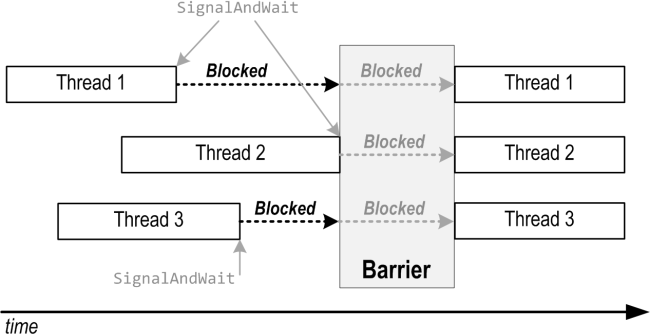
\includegraphics[scale=2]{img/barrier.png}
\end{figure}

On utilise un mutex[lock|unlock], la fonction cnd\_t[wait|signal].\\
cnd\_signal(\&c) réveille un thread.

\begin{minted}[frame=single]{c}
	int compteur = 0;
	const N = 42;
	mtx_t m;
	cnd_t c;
	barriereN(){
		mtx_lock();
		compteur++;
		while(compteur < N){
			cnd_wait(&c, &m);
		}
		// reveil en cascade, le N+1 reveil le premier et ainsi de suite
		cnd_signal(&c); 
		mtx_unlock();
	}
\end{minted}

\section{Allocateur}
On se contente de reveiller tous les threads en attente.\\
cnd\_broadcast(\&c) reveille tous les threads.
\vspace{-0.4cm}
\begin{minted}[frame=single]{c}
	const int resource = N;
	mtx_t m;
	cnd_t c;
	allocation(int n){
		mtx_lock(&m);
		while(resource<n){
			cnd_wait(&c, &m);
		}
		resource -= n;
		mtx_unlock(&m);
	}

	liberation(int n){
		mtx_lock(&m);
		resource += n;
		cnd_broadcast(&c);
		mtx_unlock(&m);
	}
\end{minted}

\textbf{\textcolor{red}{CODE CI-DESSOUS FAUX}}\\
Dans le cas où deux threads arrivent, ils se reveillent et s'endorment entre eux avec le code suivant:
\vspace{-0.4cm}
\begin{minted}[frame=single]{c}
	const int resource = N;
	mtx_t m;
	cnd_t c;
	allocation(int n){
		mtx_lock(&m);
		while(resource<n){
			cnd_wait(&c, &m);
			cnd_signal(&c);
		}
		resource -= n;
		mtx_unlock(&m);
	}

	liberation(int n){
		mtx_lock(&m);
		resource += n;
		cnd_signal(&c);
		mtx_unlock(&m);
	}
\end{minted}

\pagebreak

\section{Producteurs Consommateurs}
\begin{figure}[h!]
	\centering
	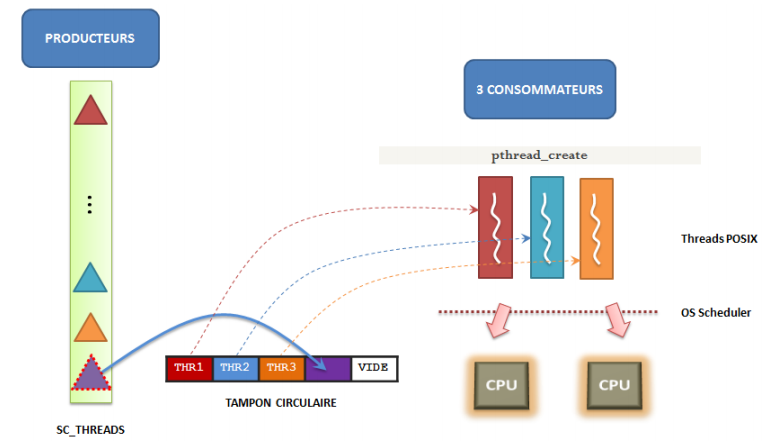
\includegraphics[scale=0.8]{img/prod_cons.png}
\end{figure}

\vspace{-0.4cm}
\begin{minted}[frame=single]{c}
	int iecr = 0; // indice d'ecriture
	int ilect = 0; // indice de lecture
	int nb = 0;
	mtx_t m;
	cnd_t fp;
	cnd_t fconso;
	Msg Tab[N];
	
	push(Msg msg){

	}

	Msg shift(){

	}
\end{minted}

\end{document}